\documentclass[11pt, a4paper, twoside]{article}

% Version en 2024 Víctor Bettachini < vbettachini@unlam.edu.ar >

\usepackage[T1]{fontenc}
\usepackage[utf8]{inputenc}

% \usepackage[spanish, es-tabla]{babel}
% \def\spanishoptions{argentina} % Was macht dass?
% \usepackage{babelbib}
% \selectbiblanguage{spanish}
% \addto\shorthandsspanish{\spanishdeactivate{~<>}}

\usepackage{graphicx}
\graphicspath{{../figuresLaTeX/}}
% \usepackage{float}

\usepackage[arrowdel]{physics}
\newcommand{\pvec}[1]{\vec{#1}\mkern2mu\vphantom{#1}}
% \usepackage{units}
\usepackage[separate-uncertainty= true, multi-part-units= single, range-units= single, range-phrase= {~a~}, locale= FR]{siunitx}
\usepackage{isotope} % $\isotope[A][Z]{X}\to\isotope[A-4][Z-2]{Y}+\isotope[4][2]{\alpha}

\usepackage{tasks}
\usepackage[inline]{enumitem}
% \usepackage{enumerate}

\usepackage{hyperref}

% \usepackage{amsmath}
% \usepackage{amstext}
% \usepackage{amssymb}

\usepackage{tikz}
\usepackage{tikz-3dplot}
\usepackage{tikz-dimline}
\usetikzlibrary{calc}
% \usetikzlibrary{math}
\usetikzlibrary{arrows.meta}
\usetikzlibrary{snakes}
\usetikzlibrary{decorations}
\usetikzlibrary{decorations.pathmorphing}
\usetikzlibrary{patterns}

\usepackage[hmargin=1cm,vmargin=3cm, top= 0.75cm,nohead]{geometry}

\usepackage{lastpage}
\usepackage{fancyhdr}
\pagestyle{fancyplain}
\fancyhf{}
\setlength\headheight{28.7pt} 
\fancyhead[LE, LO]{\textbf{Computational Analytical Mechanics} }
% \fancyhead[LE, LO]{\textbf{Mecánica General} }
\fancyhead[RE, RO]{\href{https://ingenieria.unlam.edu.ar/}{$\vcenter{\hbox{\includegraphics[height=1cm]{ambos.pdf}}}$}}
\fancyfoot{\href{https://creativecommons.org/licenses/by-nc-sa/4.0/}{$\vcenter{\hbox{\includegraphics[height=0.4cm]{by-nc-sa_80x15.pdf}}}$} \href{https://ingenieria.unlam.edu.ar/}{DIIT - UNLaM}}
\fancyfoot[C]{ {\tiny Updated \today} }
\fancyfoot[RO, LE]{Page \thepage/\pageref{LastPage}}
\renewcommand{\headrulewidth}{0pt}
\renewcommand{\footrulewidth}{0pt}


\begin{document}
\begin{center}
  \textsc{\large Constraint forces | Lagrange multipliers} 
\end{center}

\begin{enumerate}

	\item
	\begin{minipage}[t][1.1cm]{0.75\textwidth}
		\textbf{Ideal pendulum}\\
		Calculate the tension in the string using the method of Lagrange multipliers.
		The constraint is that the bead is always at \(\vec{r} = \ell \hat{\rho}\), ergo, the function expressing this is \(f(\rho) = \rho - \ell = 0\).
	\end{minipage}
	\begin{minipage}[c][0cm][t]{0.25\textwidth}
		\begin{tikzpicture}[scale= 1.0]
  		\draw [arrows=-latex] (-1,2) -> (-1,1) node [above=15, right=2] {\(\vec{g}\)}; 
			\draw [ultra thick] (-1.5,3) -- (2,3);
			\fill [pattern = north east lines] (-1.5,3) rectangle (2,3.2); 
			\draw [dashed] (0,3) -- (0,-.25);
			\draw [thick] (0,3) -- +(-60:3) node[midway,above,right=2] {\(\ell\)};	
			\shade [ball color=black!80] ($(0,3)+(-60:3)$) circle(0.25) node [] {\color{white} $m$};
    	\draw [arrows=-latex] (0,.4) -> (1.25,.4) node [midway, above] {\( \psi \)}; 
			\draw [arrows=-latex] (0,0) arc [start angle=-90, end angle=-65, radius=3] node [below=12, left=8] {\( \varphi \)};
		\end{tikzpicture}
	\end{minipage}



	\item 
	\begin{minipage}[t][4cm]{0.47\textwidth}
	\textbf{Cylinder rolling over an inclined plane} [Marion ex. 7.5]\\
		\begin{enumerate}
			\item Write the equations of motion,
			\item find the angular acceleration,
			\item and the constraint forces.
		\end{enumerate}
	\end{minipage}
	\begin{minipage}[c][2.5cm][t]{0.3\textwidth}
		\includegraphics[width=\textwidth]{figures/marion_fig6_7}
	\end{minipage}

	
	\item
	\begin{minipage}[t][6.5cm]{0.65\textwidth}
	\textbf{Double Atwood machine} [Marion ex. 7.8 and 7-37]\\
	Use the frame of reference shown in the figure.
	For this system of pulleys, determine: 
	\begin{enumerate}
		\item the equations of motion,
		\item and the tensions in both strings using the method of Lagrange multipliers.
	\end{enumerate}
	Results:\\
	\(
		Q_{1} = \frac{g \left(32 m_{1} m_{2} m_{3} + 8 m_{1} m_{2} m_{p} + 20 m_{1} m_{3} m_{p} + 4 m_{1} m_{p}^{2} + 8 m_{2} m_{3} m_{p} + 2 m_{2} m_{p}^{2} + 4 m_{3} m_{p}^{2} + m_{p}^{3}\right)}{4 m_{1} m_{2} + 4 m_{1} m_{3} + 2 m_{1} m_{p} + 16 m_{2} m_{3} + 6 m_{2} m_{p} + 14 m_{3} m_{p} + 3 m_{p}^{2}}
	\)\\
	\(
		Q_{2} = \frac{g m_{3} \cdot \left(16 m_{1} m_{2} + 6 m_{1} m_{p} + 4 m_{2} m_{p} - m_{p}^{2}\right)}{4 m_{1} m_{2} + 4 m_{1} m_{3} + 2 m_{1} m_{p} + 16 m_{2} m_{3} + 6 m_{2} m_{p} + 14 m_{3} m_{p} + 3 m_{p}^{2}}
	\)
	\end{minipage}
	\begin{minipage}[c][0.5cm][t]{0.3\textwidth}
		\includegraphics[width=\textwidth]{figures/marion_fig7_6}
	\end{minipage}


	\item
	\begin{minipage}[t][6cm]{0.65\textwidth}
		\textbf{Weights linked by a rope} [Taylor 7.50]\\
		A particle of mass \(m\) that lies over a table is linked to another particle of mass \(M\) by a rope of length \(l\) that passes through a hole in the table, without friction.
		The second one is hanging vertically at a distance \(y = \ell - \rho\) from the table, where \(\rho\) is the distance between the first particle and the hole.
		\begin{enumerate}
			\item Assuming that \(\theta\) is not necessarily constant, find the Lagrange equations for \(\rho\) and \(y\). Result:\\ \(- M g + M \ddot{y} + \lambda_{1} = 0 \qquad \lambda_{1} - m \rho \dot{\theta}^{2} + m \ddot{\rho} = 0\)
			\item Solve the system for \(\rho, y\) and the lagrange multiplier \(\lambda_1\) finding the tensions exerted upon both particles.\\
			Result: \(Q_{\rho} = \frac{M m \left(g + \rho \dot{\theta}^{2}\right)}{M + m}\)
		\end{enumerate}
	\end{minipage}
	\begin{minipage}[c][0cm][t]{0.3\textwidth}
		\includegraphics[width=\textwidth]{figures/cmchap6_fig6_5}
	\end{minipage}


	\item
	\begin{minipage}[t][4.5cm]{0.62\textwidth}
		\textbf{Particle slidding over a semi-sphere} [Marion ex. 7.10]\\
		The particle of mass \(m\), considered as a point particle, slides over a semi-sphere of radius \(R\) without friction.
		\begin{enumerate}
			\item Find the constraint force.\\
			Result: \(F^\mathrm{constraint}_{\rho} = m \left(- R \dot{\theta}^{2} + g \cos{\left(\theta \right)}\right)\)
			\item Calculate the angle at which the particle leaves the semi-sphere.\\
			Result: \(\approx 48.19^\circ\) 
		\end{enumerate}
	\end{minipage}
	\begin{minipage}[c][0cm][t]{0.3\textwidth}
		\begin{tikzpicture}[scale= 1.0]
			\draw [ultra thick] (-3,0) -- (3,0);
			\fill [pattern = north east lines] (-3,0) rectangle (3,-0.2);
			\draw [ultra thick] (-2,0) .. controls (-2,2*0.555) and (-2*0.555,2) .. (0,2) .. controls (2*0.555,2) and (2,2*0.555) .. (2,0); 
			\shade [ball color=black!80] (2*0.5+.12,1.732+.18) circle(0.2) node [] {\color{white} $m$};
			\draw [dashed] (0,0) -- (0,2);
			\draw [-LaTeX] (0,0) -- (1,1.732) node [midway, anchor=west] {\(R\)}; 
			\draw [-stealth] (0,1) arc (90:60:1) node [above left] {\(\theta\)};  
			\draw [-stealth, thick] (-2.5,2) -> (-2.5,1) node [above=15, right=2] {\(\vec{g}\)}; 
		\end{tikzpicture}
	\end{minipage}
	
	To find the angle at which the particle leaves the semi-sphere, you must solve the differential equation you'll get after working out the rather tough constraint force, which will be $\ddot{\theta} = \frac{g \sin(\theta)}{R}$.
	This expression can be integrated for the perticle's trajectory.
	This is easier after applying the chain rule to insert derivatives with respect to \(\theta\).
	$$
		\ddot{\theta} 
		= \frac{d \dot{\theta} }{d t} 
		= \frac{d \theta}{d t} \frac{d \dot{\theta}}{d \theta} 
		= \dot{\theta} \frac{d \dot{\theta}}{d \theta}
	$$

	Since the particle starts at $\theta(t=0) = 0$ with $\dot{\theta}(t=0) = 0$:
	$$
	\begin{aligned}
		\ddot{\theta} = \dot{\theta} \frac{d \dot{\theta}}{d \theta}
		&= \frac{g}{R} \sin(\theta)\\
		\dot{\theta} d \dot{\theta}
		&= \frac{g}{R} \sin(\theta) d \theta \\
		\int_0^{\dot{\theta}_\mathrm{leaving}} \dot{\theta} d \dot{\theta}
		&= \frac{g}{R} \int_0^{\theta_\mathrm{leaving}} \sin{\theta} d \theta\\
		\frac{\dot{\theta}^2}{2} \bigg|_0^{\dot{\theta}_\mathrm{leaving}}
		&= \frac{g}{R} (-\cos{\theta}) \bigg|_0^{\theta_\mathrm{leaving}}\\
		\frac{\dot{\theta}_\mathrm{leaving}^2}{2}
		&= \frac{g}{R} (-\cos(\theta_\mathrm{leaving}) + 1)\\
	\end{aligned}
	$$
	After this, you have to substitute $\dot{\theta}^2$ in an expression for $F^\mathrm{constraint}_{\rho}$, that must vanish at the moment of leaving the semi-sphere.


\end{enumerate}

\end{document}
